\documentclass[12pt,a4paper,openright,twoside]{report}

\usepackage[british]{babel}
\usepackage[utf8]{inputenc}

\usepackage{fancyhdr}
\usepackage{indentfirst}
\usepackage{graphicx}
\usepackage{newlfont}
\usepackage{xcolor}

\usepackage{stmaryrd}


\usepackage{amssymb}
\usepackage{amsmath}
\usepackage{latexsym}
\usepackage{amsthm}
\usepackage{mathabx}

\usepackage[left=1 in,right=1.4in]{geometry}

\oddsidemargin=25pt 
\evensidemargin=15pt
\hyphenation{pa-ra-me-tric}
\pagestyle{fancy}\addtolength{\headwidth}{20pt}
\renewcommand{\chaptermark}[1]{\markboth{\thechapter.\ #1}{}}
\renewcommand{\sectionmark}[1]{\markright{\thesection \ #1}{}}
\rhead[\fancyplain{}{\bfseries\leftmark}]{\fancyplain{}{\bfseries\thepage}}
\cfoot{}
\linespread{1}

% Style theorem boxes

\theoremstyle{plain}
\newtheorem{proposition}{Proposition}
\newtheorem{definition}[proposition]{Definition}
\newtheorem{conjecture}[proposition]{Conjecture}

\theoremstyle{definition}
\newtheorem{remark}[proposition]{Remark}
\newtheorem{example}[proposition]{Example}


%%%%%%%%%%%%%%%%%%%%%%%%% DEDICATION %%%%%%%%%%%%%%%%%%%%%%%%%%%%%%%%%%%%%%%

\begin{document}

\begin{titlepage}
\thispagestyle{empty}                   
\topmargin=6.5cm                        
\raggedleft                             
\large                                  
                                       
\em                                     
To my beloved\\
Benedetta                   
\newpage                                

\clearpage{\pagestyle{empty}\cleardoublepage}
\end{titlepage}
\pagenumbering{roman}


            









































%%%%%%%%%%%%%%%%%%%%%%% INTRODUCTION %%%%%%%%%%%%%%%%%%%%%%%%%%%%%%

\chapter*{Introduction}   
\addcontentsline{toc}{chapter}{Introduction}
\rhead[\fancyplain{}{\bfseries Introduction}]{\fancyplain{}{\bfseries\thepage}}\lhead[\fancyplain{}{\bfseries\thepage}]{\fancyplain{}{\bfseries Introduction}}



  \section*{English version}




  \textcolor{blue}{Machine learning literature is exploding in size and complexity, but most solutions found are ad hoc, there is little communication between different subfields, and there is a large research debt. Category theory can solve these problems.  \cite{shiebler2021category}.}

  \textcolor{blue}{Talk about the origins of category theory and its "rise to power" as a common language that aims to unite different fields of knowledge.}
    
  \textcolor{blue}{Discuss the purpose of this work: a beginner-friendly survey of categorical approaches to neural networks, causal models, and interpretability.}


  \section*{Italian version}

  \textcolor{blue}{Traduzione italiana dell'introduzione.}


\clearpage{\pagestyle{empty}\cleardoublepage}





















































%%%%%%%%%%%%%%%%%%%%%%%%%%%%% TABLE OF CONTENTS %%%%%%%%%%%%%%%%%%%%%%%%%%%%%%

\tableofcontents
\rhead[\fancyplain{}{\bfseries\leftmark}]{\fancyplain{}{\bfseries\thepage}} \lhead[\fancyplain{}{\bfseries\thepage}]{\fancyplain{}{\bfseries Table of Contents}}
\clearpage{\pagestyle{empty}\cleardoublepage}






























































%%%%%%%%%%%%%%%%%%%%%%% CATEGORICAL TOOLKIT %%%%%%%%%%%%%%%%%%%%%%%%%%%


\chapter{Categorical Toolkit}
\lhead[\fancyplain{}{\bfseries\thepage}]{\fancyplain{}{\bfseries\rightmark}}
\pagenumbering{arabic}

In this chapter, we illustrate a few categorical tools that have been developed to provide compositional frameworks for gradient-based learning and Bayesian learning. In particular, we will focus on parametric weighted optics and compositional models. Although such frameworks have been developed separately, they do interact, and they share a common philosophy: their purpose is to unify the field of machine learning and replace unreliable, non-compositional, \textit{ad hoc} tools with reliable, compositional, elegant tools.


We are forced by space and time constraints to skip over the details of many constructions, but we hope the reader can get a good picture of how the proposed tools work. All the necessary details can be found in the cited references.


Note that this chapter is devoted to illustrating our categorical toolkit itself, not its applications. Hence, we will focus on the mathematical and categorical aspects of the presented frameworks, and we will postpone applications to the following chapters.

\section{Parametric weighted optics}

Neural networks have two main properties: they depend on parameters and information flows through them bidirectionally (forward propagation and back propagation). Any aspiring categorical model of neural networks must take these two aspects into consideration: the framework of parametric weighted optics (see \cite{gavranovic2024fundamental} for a thorough and mostly novel treatment of the subject and see \cite{cruttwell2022categorical} for experimental results) does just that, as it offers bidirectionality using weighted optics and parametrization using the $\mathbf{Para}$ construction.
In this section, we will sketch out the construction of this framework loosely following \cite{gavranovic2024fundamental}.

\subsection{Parametric categories}

In this section, we will focus on parametric and coparametric categories. While the use case for parameters is obvious to any machine learning practitioner, one might ask why coparameters are even useful. As we will see, coparameters will come very handy in building parametric weighted optics.


\subsubsection{Actegories}

Before we can deal with (co)parametric maps, we need to find a way to glue input/output spaces to parameter spaces, so that such maps have well-defined (co)domains. One common strategy is to provide the category at hand with a monoidal structure. However, monoidal products can only combine elements within the same underlying category. Since (co)parameters are often taken from spaces that are different in nature from the input and output spaces, a more general mathematical tool is needed: namely, actegories (see the survey \cite{capucci2022actegories} for a thorough treatment of the subject). 


Actegories are actions of symmetric monoidal categories on other categories. For brevity's sake, we will only give an incomplete definition (see \cite{capucci2022actegories} or \cite{gavranovic2024fundamental} for complete definitions).

\begin{definition}[Actegory]
  Let $(\mathcal{M},I,\otimes)$ be a monoidal category. A (right) $\mathcal{M}$-actegory is a tuple $(\mathcal{C}, \bullet, \eta, \mu)$, where:
  \begin{enumerate}
    \item $\mathcal{C}$ is a category;
    \item $\bullet: \mathcal{C} \times \mathcal{M} \to \mathcal{C}$ is a functor;
    \item $\eta$ and $\mu$ are natural isomorphisms satisfying the diagrams in ADDIM.
  \end{enumerate}
  The natural isomorphisms $\eta$ and $\mu$ must also satisfy coherence conditions. If $\eta$ and $\mu$ are identical transformations, we say that the actegory is strict.
\end{definition}

Thus, if we want a map $A \to B$ with parameters in $P$, we will find an appropriate actegory and an appropriate map $A \bullet P \to B$.

\begin{remark}
  The definition of actegory given above technically pertains right actegories: left actegories are defined analogously.
\end{remark}

We will also be interested in actegories that interact with the monoidal structure of the underlying category.

\begin{definition}[Monoidal actegory]
  Let $(\mathcal{M},I,\otimes)$ be a braided monoidal category and let $(\mathcal{C}, \bullet, \eta, \mu)$ be an actegory. Suppose $\mathcal{C}$ has a monoidal structure $(J,\boxtimes)$. Then we say that $(\mathcal{C}, \bullet)$ is monoidal if the underlying function $\bullet$ is strong monoidal and the transformation $\eta$ and $\mu$ are also monoidal.
\end{definition}



\subsubsection{The $\mathbf{Para}$ construction}


Suppose we have an $\mathcal{M}$-actegory $(\mathcal{C}, \bullet)$. We wish to study maps in $\mathcal{C}$ which are parametrized using objects of $\mathcal{M}$. We are not just interested in the maps by themselves, but also in their compositional structure. Thus, we abstract away the details by defining a new category $\mathbf{Para}_{\bullet}(\mathcal{C})$ (first defined in \cite{fong2019backprop}). Since we also want to formalize the role of reparametrization, we actually construct $\mathbf{Para}_{\bullet}(\mathcal{C})$ as a bicategory, so that its $0$-cells can serve as input/output spaces, and its $1$-cells can serve as parametric maps, and, finally, its $2$-cells can serve as parameter changes.

\begin{definition}[$\mathbf{Para}_{\bullet}(\mathcal{C})$]
  Let $(\mathcal{C}, \bullet)$ be a right $\mathcal{M}$-actegory. Then, we define $\mathbf{Para}_{\bullet}(\mathcal{C})$ as the bicategory whose components are as follows.
  \begin{itemize}
    \item The $0$-cells are the objects of $\mathcal{C}$.
    \item The $1$-cells are pairs $(P,f): A \to B$, where $P : \mathcal{C}$ and $f: A \bullet P \to B$.
    \item The $2$-cells come in the form $r: (P,f) \Rightarrow (Q,g)$, where $r: P \to Q$ is a morphism in $\mathcal{C}$. $r$ must also satisfy a naturality condition.
    \item The $1$-cell composition law is
    \[(P,f) \fatsemi (Q,g) = (P \otimes Q, f \bullet Q \fatsemi g).\]
    \item The horizontal and vertical $2$-cell composition laws are respectively given by parallel and sequential products in $\mathcal{M}$. 
  \end{itemize}
  It is quite handy to represent such cells using the string diagram notation illustrated in figure ADDIM.
\end{definition}


It is shown in \cite{gavranovic2024fundamental} that $\mathbf{Para}_{\bullet}(\mathcal{C})$ is actually a $2$-category if the underlying actegory is strict. Assuming this is the case, we can use a functor $F: \mathbf{Cat} \to \mathbf{Set}$ to quotient out the $2$-categorical structure and turn $\mathbf{Para}_{\bullet}(\mathcal{C})$ into a $1$-category $F_{*}(\mathbf{Para}_{\bullet}(\mathcal{C}))$. Here, $F_{*}: \mathbf{2Cat} \to \mathbf{Set}$ is the change of enrichment basis functor induced by $F$. We will see the significance of this construction later.


The $\mathbf{Para}$ construction has a dual $\mathbf{coPara}$ construction which is designed to represent coparametric morphisms. The main differences between the two constructions are that $(\mathcal{C}, \bullet)$ is required to be a left actegory this time, and that $1$-cells $A \to B$ in $\mathbf{coPara}_{\bullet}(\mathcal{C})$ take the form $(P,f)$, where $f: A \to P \bullet B$.
Cells in $\mathbf{coPara}_{\bullet}(\mathcal{C})$ can also be represented with appropriate string diagrams (see ADDIM). The reader can find a complete definition in \cite{gavranovic2024fundamental}.


Both $\mathbf{Para}_{\bullet}(\mathcal{C})$ and $\mathbf{coPara}_{\bullet}(\mathcal{C})$ can be given a monoidal structure if $(\mathcal{C}, \bullet)$ is a monoidal actegory. This is extremely important because it allows us to compose (co)parametric morphisms both in sequence and in parallel. Once again, more detail can be found in \cite{gavranovic2024fundamental}.


\begin{remark}
  Another way to parametrize morphisms is the coKleinsli construction. As noted by \cite{gavranovic2024fundamental}, the main difference between $\mathbf{coKl}$ and $\mathbf{Para}$ is that the parametrization offered by $\mathbf{coKl}$ is global, while the parametrization offered by $\mathbf{Para}$ is local: all morphisms in $\mathbf{coKl}(X \times -)$ must take a parameter in $X$, while the parameter space of different morphisms of $\mathbf{Para}(\mathcal{C})$ admit different parameter spaces. Nevertheless, the two constructions are relate, and the former can be embedded into the latter.
\end{remark}




\subsection{Bidirectionality through optics}

Modelling bidirectional flows of information is not only useful in machine learning, but also in game theory, database theory, and more. As such, categorical tools for bidirectionality have been sought after for a long time: in particular, the greatest deal of efforts has been devoted to developing lens theory. Lenses have then been generalized into optics (see e.g. \cite{riley2018categories}) to subsume other tools such as prisms and traversals into the same framework. Finally, there have also been various attempts at generalizing optics (see e.g. \cite{clarke2024profunctor} for a definition of mixed optics). We will introduce lenses and optics, and focus on the generalization of optics that appears (to us) to be the most versatile: weighted optics (first introduced in \cite{gavranovic2024fundamental}). 


\subsubsection{Lenses}

As stated in \cite{gavranovic2024fundamental}, there is no standard definition of lens, and different authors opt for different \textit{ad hoc} definitions that best suit their purposes. We will borrow the perspective of \cite{cruttwell2022categorical} and give the following definition.


\begin{definition}[Lenses]
  \label{def: lenses}
  Let $\mathcal{C}$ be a Cartesian category. Then, $\mathbf{Lens}(\mathcal{C})$ is the category defined by the following data:
  \begin{itemize}
    \item an object of $\mathbf{Lens}(\mathcal{C})$ is a pair $\left(\begin{smallmatrix} A \\ A' \end{smallmatrix}\right)$ of objects in $\mathcal{C}$; 
    
    \item a $\left(\begin{smallmatrix} A \\ A' \end{smallmatrix}\right) \to \left(\begin{smallmatrix} B \\ B' \end{smallmatrix}\right)$ morphism (or lens) is a pair $\left(\begin{smallmatrix} f \\ f' \end{smallmatrix}\right)$ of morphisms of $\mathcal{C}$ such that $f: A \to B$ and $f': A \times B' \to A'$. $f$ is known as the forward pass of the lens $\left(\begin{smallmatrix} f \\ f' \end{smallmatrix}\right)$, whereas $f'$ is known as the bacward pass;
    
    \item given $\left(\begin{smallmatrix} A \\ A' \end{smallmatrix}\right) : \mathbf{Lens}(\mathcal{C})$, the associated identity lens is $\left(\begin{smallmatrix} 1_A \\ \pi_1 \end{smallmatrix}\right)$;
    
    \item the composition of $\left(\begin{smallmatrix} f \\ f' \end{smallmatrix}\right): \left(\begin{smallmatrix} A \\ A' \end{smallmatrix}\right) \to \left(\begin{smallmatrix} B \\ B' \end{smallmatrix}\right)$ and $\left(\begin{smallmatrix} g \\ g' \end{smallmatrix}\right): \left(\begin{smallmatrix} B \\ B' \end{smallmatrix}\right) \to \left(\begin{smallmatrix} C \\ C' \end{smallmatrix}\right)$ is
    \[\left(\begin{smallmatrix} f \fatsemi g \\ \langle \pi_0, \langle \pi_0 \fatsemi f, \pi_1 \rangle \fatsemi g' \rangle \fatsemi f' \end{smallmatrix}\right).\]
  \end{itemize}
\end{definition}


Lenses are best thought of in the helpful language of the string diagrams illustrated in ADDIM. For instance, the composition formula in the definition above looks very complicated, but its graphical counterpart shown in ADDIM is extremely intuitive.


As we will soon see, in machine learning, the forward pass of a lens is used to model forward propagation, whereas the associated backward pass is tasked with modelling backpropagation. In other contexts, such as functional programming, lenses are used as data accessors for objects: the forward pass serves as a getter, while the backward pass serves as a setter (see e.g. \cite{steckermeier2015lenses}).


\subsubsection{Optics}

Lenses are a powerful tool, but they cannot be used to model all situations: for instance, lenses cannot be used if we wish to be able to choose not to interact with the environment depending on the input, or if we wish like to reuse values computed in the forward pass for further computation in the backward pass.


Optics generalize lenses by weakening the link between \textsc{get} maps and \textsc{put} maps and by replacing the Cartesian structure of the underlying category with a simpler symmetric monoidal structure. In an optic over $\mathcal{C}$, an object $M : \mathcal{C}$ acts as an inaccessible residual space transferring information between the upper components and the lower component.
We will provide the definition given by \cite{riley2018categories}, but we will use the string diagram notation presented by \cite{gavranovic2024fundamental} for the sake of consistency.

\begin{definition}[Optics]
  Let $(\mathcal{C}, I, \otimes, \lambda, \rho, \alpha)$ be a symmetric monoidal category (we make the unitors and associators explicit for later use). Then, $\mathbf{Optic}(\mathcal{C})$ is the category defined by the following data:
  \begin{itemize}
    \item an object of $\mathbf{Optic}(\mathcal{C})$ is a pair $\left(\begin{smallmatrix} A \\ A' \end{smallmatrix}\right)$ of objects in $\mathcal{C}$; 
    \item a $\left(\begin{smallmatrix} A \\ A' \end{smallmatrix}\right) \to \left(\begin{smallmatrix} B \\ B' \end{smallmatrix}\right)$ morphism (or optic) is a pair $\left(\begin{smallmatrix} f \\ f' \end{smallmatrix}\right)$ of morphisms of $\mathcal{C}$ such that $f: A \to M \otimes B$ and $f': M \otimes B' \to A'$, where $M : \mathcal{C}$ is known as residual space; such pairs $\left(\begin{smallmatrix} f \\ f' \end{smallmatrix}\right)$ are also quotiented by an equivalence relation that allows for reparametrization of the residual space and effectively makes it inaccessible;
    \item the identity on $\left(\begin{smallmatrix} A \\ A' \end{smallmatrix}\right)$ is the optic represented by $(\lambda_A^{-1}, \lambda_A)$.
  \end{itemize}
\end{definition}

We will only show how optics compose using the string diagrams in ADDIM (see \cite{riley2018categories} for the composition formula).

\begin{remark}
  A more versatile but also more mathematically sophisticated definition of optics relies on coends. Under the coend formalism,
  \[\mathbf{Optic}(\mathcal{C})\left(\left(\begin{smallmatrix} A \\ A' \end{smallmatrix}\right),\left(\begin{smallmatrix} B \\ B' \end{smallmatrix}\right)\right) = \int^{M : \mathcal{C}}\mathcal{C}(A,M \times B) \times \mathcal{C}(M \otimes B',A').\] 
  See \cite{riley2018categories} for more information about this topic.
\end{remark}

Lenses come up as a special case of optics (\cite{riley2018categories}), and optics do solve some of the issues we have with lenses. However, optics are not perfect either: for instance, \cite{gavranovic2024fundamental} points out that optics cannot be used in cases where we ask that the forward pass and backward pass are different kind of maps, as they are both forced to live in the same category. Thus, we need a further layer of generalization: namely, weighted optics.



\subsubsection{Category of elements of a functor}

Before we define weighted optics, we need to introduce a new tool to our toolbox: the category of elements of a functor.

\begin{definition}[Elements of a functor]
  Let $F: \mathcal{C} \to \mathbf{Set}$ be a functor. We define $\mathbf{El}(F)$ as the category with the following data: (i) the objects of $\mathbf{El}(F)$ are pairs $(C, x)$ where $C : \mathcal{C}$ and $x : F(C)$; (ii) the $(C, x) \to (D, y)$ morphisms in $\mathbf{El}(F)$ are the morphisms $f: C \to D$ in $\mathcal{C}$ such that $F(f)(x) = y$.
\end{definition}

\cite{gavranovic2024fundamental} studies $\mathcal{B}$-actegories $(\mathcal{C}, \bullet)$, which are then reparametrized so that the acting category becomes $\mathcal{E} = \mathbf{El}(W)$ for some weight functor $W: \mathcal{B}^{\mathrm{op}} \to \mathbf{Set}$ (which is to be specified). The reparametrization takes place thanks to the opposite of the forgetful functor $\pi_W: \mathcal{E} \to \mathcal{B}^{\mathrm{op}}$, which maps $(B,x) \mapsto B$. Hence, we consider the action
\[\bullet^{\pi_W^{\mathrm{op}}} = \mathbf{El}(W)^{\mathrm{op}} \times \mathcal{C} \stackrel{\pi_W^{\mathrm{op}} \times \mathcal{C}}{\longrightarrow} \mathcal{B} \times \mathcal{C} \stackrel{\bullet}{\longrightarrow} \mathcal{C}.\]
\cite{gavranovic2024fundamental} also gives the following definition, which is later instrumental in defining weighted lenses.

\begin{definition}[Weighted $\mathbf{coPara}$]
  If $W$ is a weight functor as above and $(\mathcal{C}, \bullet)$ is a $\mathcal{B}$-actegory, we define
  \[\mathbf{coPara}^W_{\bullet}(\mathcal{C}) = \pi_{0*}(\mathbf{coPara}_{\bullet^{\pi_W^{\mathrm{op}}}}(\mathcal{C})),\]
  where $\pi_{0*}$ is the enrichment base change functor generated by the connected component functor $\pi_{0}: \mathbf{Cat} \to \mathbf{Set}$. More explicitly, $\pi_{0*}$ quotients the connections provided by reparametrizations.
\end{definition}



\subsubsection{Weighted optics}

We are finally ready to define weighted optics.

\begin{definition}[Weighted optics]
  Suppose $(\mathcal{C}, \bullet)$ is an $\mathcal{M}$-actegory, suppose $(\mathcal{D}, \sqbullet)$ is an $\mathcal{M}'$-actegory, and suppose $W: \mathcal{M}^{\mathrm{op}} \times \mathcal{M}' \to \mathbf{Set}$ is a lax monoidal functor.
  We define the category of $W$-weighted optics over the product actegory $\left(\mathcal{C}\times\mathcal{D}^{\mathrm{op}},\left(\begin{smallmatrix}\bullet\\\sqbullet^{\mathrm{op}}\end{smallmatrix}\right)\right)$ as
  \[\mathbf{Optic}^W_{\left(\begin{smallmatrix}\bullet\\\sqbullet\end{smallmatrix}\right)} = \mathbf{coPara}^W_{\left(\begin{smallmatrix}\bullet\\\sqbullet^{\mathrm{op}}\end{smallmatrix}\right)}(\mathcal{C}\times\mathcal{D}^{\mathrm{op}}).\]
\end{definition}

The definition is very dense and deserves some explanation. Fist of all, we assume that $W$ maps $(M,M')$ to a set of maps $s: M \to M'$. If that's the case, a $\left(\begin{smallmatrix}X\\X'\end{smallmatrix}\right) \to \left(\begin{smallmatrix}Y\\Y'\end{smallmatrix}\right)$ map is a triplet $\left(\left(\begin{smallmatrix}\\M'\end{smallmatrix}\right),s,\left(\begin{smallmatrix}f\\f'\end{smallmatrix}\right)\right)$, where $M$ is the forward residual, $M'$ is the backward residual, $s: M \to M'$ links the two residuals, $f: X \to M \bullet Y$ is the forward pass, and $f': M' \bullet Y' \to X'$ is the backward pass.
The triplets are also quotiented with respect to reparametrization, which makes the residual spaces effectively inaccessible (as it happens in the case of ordinary optics).


A weighted optic is a rather sophisticated piece of categorical machinery, but we can get a clear "functional" understanding of how it works looking at an associated string diagram: data from $X$ flows through the forward map, which computes an output in $Y$ and a forward residual in $M$. Such forward residual is the converted into a backward residual in $M'$ by the map $s$, which is provided by the weight functor. Then, the backward residual is used to compute, together with input from $Y'$ a value in $X'$. The last step happens thanks to the backward map $f'$. The composition law is just as complicated as the optics, but it is not difficult to understand if considered from the point of view of string diagrams: see, for instance, ADDIM. More information can be found on \cite{gavranovic2024fundamental}.


\begin{remark}
  Weighted optics can also be defined using coend calculus: it is shown in \cite{gavranovic2024fundamental} that:
  \[\mathbf{Optic}^W_{\left(\begin{smallmatrix}\bullet\\\sqbullet\end{smallmatrix}\right)}\left(\begin{matrix} A \\ A'\end{matrix},\begin{matrix} B \\ B'\end{matrix}\right) \cong \int^{(M,M') : \mathcal{M} \times \mathcal{M}'}\mathcal{C}(A, M \bullet B) \times W(M,M') \times \mathcal{D}(M' \sqbullet B', A').\]
\end{remark}


The advantages of weighted optics over ordinary optics are clear: when dealing with weighted optics, we are no longer forced to take reverse maps from the same category as the forward maps. The action on the category of forward spaces is now separated from the action on the category of backward spaces, and the link between the two actions is provided by an external functor. Such modular approach provides a great deal of conceptual clarity and flexibility, more than regular optics or lenses can provide on their own.


As stated in \cite{gavranovic2024fundamental}, since $\mathbf{coPara}$ can be given a monoidal structure, we can also give $\mathbf{Optic}^W_{\left(\begin{smallmatrix}\bullet\\\sqbullet\end{smallmatrix}\right)}$ one such structure as long as the underlying actegories are monoidal and the weight functor $W$ is braided monoidal.


It is also shown in \cite{gavranovic2024fundamental} that weighted optics are indeed a generalization of optics. In particular, it is shown that the lenses in \textit{Def. \ref{def: lenses}} are the specialized weighted optics obtained when $\mathcal{C} = \mathcal{D}$ is Cartesian and the actegories are given by the Cartesian product. More generally, the thesis claims that - to the best of the author's knowledge - all definitions of lenses currently used in the literature are subsumed by the definition of weighted optics.



\subsubsection{Parametric weighted optics}

Although weighted optics model bidirectionality very well, they cannot be used to model neural networks just yet, as they are not parametric objects. The $\mathbf{Para}$ construction can only be applied to weighted optics if we find an appropriate action on $\mathbf{Optic}^W_{\left(\begin{smallmatrix}\bullet\\\sqbullet\end{smallmatrix}\right)}$. As shown in \cite{gavranovic2024fundamental}, this can be done under the assumption that $\mathcal{M}$ and $\mathcal{M}'$ are braided: if that's the case, we can just weighted optic category $ \mathcal{V} = \mathbf{Optic}^W_{\left(\begin{smallmatrix}\otimes\\\otimes'\end{smallmatrix}\right)}$ generated by the self-actions of the two categories, and we can define a $\mathcal{V}$-action $\Asterisk$ on $\mathbf{Optic}^W_{\left(\begin{smallmatrix}\bullet\\\sqbullet\end{smallmatrix}\right)}$ so that 
\[\left(\begin{matrix}M\\M'\end{matrix}\right) \Asterisk \left(\begin{matrix}X\\X'\end{matrix}\right) = \left(\begin{matrix}M \bullet X\\ M' \sqbullet X'\end{matrix}\right).\]
We can then write the following definition:

\begin{definition}[Parametric weighted optics]
  Let $(\mathcal{M}, I, \otimes)$ and let $(\mathcal{M}', I', \otimes')$ be braided monoidal categories. Let $(\mathcal{C}, \bullet)$ and $(\mathcal{D}, \sqbullet)$ be an $\mathcal{M}$-actegory and an $\mathcal{M}'$-actegory, respectively. Finally, let $F: \mathcal{M} \to \mathcal{M}'$ be a lax monoidal functor. Then, if $\Asterisk$ is the action mentioned above, we define the category of parametric weighted optics as 
  \[\mathbf{Para}_{\Asterisk}\left(\mathbf{Optic}^W_{\left(\begin{smallmatrix}\bullet\\\sqbullet\end{smallmatrix}\right)}\right).\]
\end{definition}

Parametric weighted optics are an even more sophisticated piece of categorical machinery than non-parametric ones, and thus the consistent use of string diagrams is extremely helpful. Refer to ADDIM to see examples of such diagrams.





\subsection{Differential categories}
\label{subsec: diffcats}


Modelling gradient-based learning obviously requires a setting where differentiation can take place. Although it is tempting to directly employ Euclidean space, recent research has shown that there are tangible advantages in working with generalized differential combinators that extend the notion of derivative to polynomial circuits (\cite{wilson2022categories}, \cite{wilson2021reverse}), manifolds (ADDREF), complex spaces (ADDREF), and so on. 
Thus, it makes sense to work with an abstract notion of derivative which can then be implemented as a known differential combinator through the choice of an appropriate differential category.


\subsubsection{The standard approach to differential categories}


The first two abstract settings for differentiation that we consider are Cartesian differential categories (first introduced in \cite{blute2006differential}) and Cartesian reverse differential categories (first introduced by \cite{cockett2019reverse}). The former allow for forward differentiation, while the latter allow for reverse differentiation. We will omit the defining axioms for the sake of brevity, but the reader can find complete definitions in \cite{cockett2019reverse}.

\begin{definition}[Cartesian differential category]
  A Cartesian differential category (CDR) $\mathcal{C}$ is a Cartesian left-additive category where a differential combinator $\mathrm{D}$ is defined. Such differential combinator must take a morphism $f: A \to B$ and return a morphism $\mathrm{D}[f]: A \times A \to B$, which is known as the derivative of $f$. The combinator $\mathrm{D}$ must satisfy a number of axioms. 
\end{definition}

\begin{definition}[Cartesian reverse differential category]
  A Cartesian reverse differential category (CRDC) $\mathcal{C}$ is a Cartesian left-additive category where a reverse differential combinator $\mathrm{R}$ is defined. Such reverse differential combinator must take a morphism $f: A \to B$ and return a morphism $\mathrm{R}[f]: A \times B \to A$, which is known as the reverse derivative of $f$. The combinator $\mathrm{R}$ must satisfy a number of axioms. 
\end{definition}


The aforementioned axioms make sure that $\mathrm{D}$ and $\mathrm{R}$ satisfy the properties expected from derivative and reverse derivative. In particular, a differential combinator satisfies a chain rule (see figure ADDIM), whereas a reverse differential combinator satisfies a reverse chain rule (see figure ADDIM).


\begin{example}
  $\mathbf{Smooth}$ is a both a CDC and a CRDC. In fact, if $\mathcal{J}_f$ is the Jacobian matrix of a smooth morphism $f$,
  \[\mathrm{D}[f]: (x,v) \mapsto \mathcal{J}_f(x)v\]
  and
  \[\mathrm{R}[f]: (x,y) \mapsto \mathcal{J}_f(x)^Ty\]
  induce well-defined combinators $\mathrm{D}$ and $\mathrm{R}$. This is only a partial coincidence, as shown in \cite{cockett2019reverse} that CRDCs are always CDCs under a canonical choice of differential combinator. The converse, however, is generally false.
\end{example}


As it turns out, forward differentiation tends to be less efficient when dealing with neural networks that come up in practice, so CDCs are not extremely useful when studying deep learning. CRDCs, on the other hand, have been applied to great success (see e.g. \cite{cruttwell2022categorical}). Moreover, CRDCs have been recently generalized by \cite{gavranovic2024fundamental} to coalgebras associated with copointed endofunctors. We will examine the generalized definition later on.



\subsubsection{The $\mathbf{Lens}_A$ construction}


It is shown in \cite{gavranovic2024fundamental} that there is a particular class of weighted optics which is useful for reverse differentiation, being able to represent both maps (through forward passes) and the associated reverse derivatives (through backward passes). Moreover, such weighted optics can be represented as lenses in the sense of \textit{Def \ref{def: lenses}}, which means that their inner workings can be pictured in a simple, intuitive way.
Let us start by defining a new kind of Cartesian left-additive category.


\begin{definition}[Additively closed Cartesian left-additive category]
  A Cartesian left-additive category $\mathcal{C}$ is an additively closed Cartesian left-additive category (ACCLAC) if and only if the following are true:
  \begin{itemize}
    \item the subcategory $\mathbf{CMon}(\mathcal{C})$ of additive maps has a closed monoidal structure $(I, \otimes)$;
    \item the embedding $\iota: \mathbf{CMon}(\mathcal{C}) \to \mathcal{C}$ is a lax monoidal funtor with respect to the aforementioned structure of $\mathbf{CMon}(\mathcal{C})$ and the Cartesian structure of $\mathcal{C}$.
  \end{itemize}
\end{definition}


Then, we can define the category of lenses with backward passes additive in the second component.

\begin{definition}
  Let $\mathcal{C}$ be an ACCLAC with Cartesian structure is $(1, \times)$ and whose subcategory $\mathbf{CMon}(\mathcal{C})$ has monoidal structure $(I, \otimes)$. Then, we define
  \[\mathbf{Lens}_A(\mathcal{C}) = \mathbf{Optic}_{\left(\begin{smallmatrix}\times \\ \otimes\end{smallmatrix}\right)}^{\mathcal{C}(-,\iota(-))}.\]
\end{definition}

As argued in \cite{gavranovic2024fundamental}, the symbol $\mathbf{Lens}_A$ is justified because one such optic of type $\left(\begin{smallmatrix}X \\ X'\end{smallmatrix}\right) \to \left(\begin{smallmatrix}Y \\ Y'\end{smallmatrix}\right)$ can be concretely represented as a lens with forward pass $f : \mathcal{C}(X,Y)$ and backward pass $f' : \mathcal{C}(X \times Y',X')$. We do not have the space to report the details of this argument, but we report the following remark.

\begin{remark}
  Some potential expressiveness is lost when passing from weighted optic composition to concrete lens composition. In particular, if we operated with optics, we would be able to implement backpropagation without resorting to gradient checkpointing, which is not possible if we use lenses. 
\end{remark}


\cite{gavranovic2024fundamental} proposes the following conjecture.

\begin{conjecture}
  Weighted optics provide good denotational and operational semantics for differentiation.
\end{conjecture}

Since the conjecture hasn't been formally proved yet, the author abandons the weighted optics perspective in favor of the lens perspective, and so do we. As it has already been shown in \cite{cruttwell2022categorical}, lenses are expressive enough to satisfyingly model gradient based learning, and thus, while weighted optics seem to offer great future potential, lens-theoretic approaches are far from being disadvantageous.


\subsubsection{}





\subsubsection{Generalized reverse differential categories}

\cite{gavranovic2024fundamental} proposes the $\mathbf{Lens}_A$ construct as foundation for generalizing reverse differential categories. This is possible because $\mathbf{Lens}_A$ is an endofunctors, as shown by the following definitions and propositions.

\begin{definition}
  We defined $\mathbf{CLACat}$ as the category whose objects are Cartesian left-additive categories and whose morphisms are Cartesian left-additive functors (see e.g.\cite{blute2006differential}).
\end{definition}

\begin{proposition}
  If $\mathcal{C} : \mathbf{CLACat}$, then $\mathbf{Lens}_A(\mathcal{C}) : \mathbf{CLACat}$.
\end{proposition}
\begin{proof}
  The Cartesian structure on $\mathbf{Lens}_A(\mathcal{C})$ is given by $\left(\begin{smallmatrix}X \\ X'\end{smallmatrix}\right) \times \left(\begin{smallmatrix}Y \\ Y'\end{smallmatrix}\right) = \left(\begin{smallmatrix}X\times Y \\ X' \times Y'\end{smallmatrix}\right)$ and by the initial object $\left(\begin{smallmatrix}1 \\ 1\end{smallmatrix}\right)$. The monoidal structure on each $\left(\begin{smallmatrix}X \\ X'\end{smallmatrix}\right)$ is given by the unit $0_{\left(\begin{smallmatrix}X \\ X'\end{smallmatrix}\right)} = \left(\begin{smallmatrix}0_A \\ !_{1 \times A'}\end{smallmatrix}\right): \left(\begin{smallmatrix}1 \\ 1\end{smallmatrix}\right) \to \left(\begin{smallmatrix}X \\ X'\end{smallmatrix}\right)$ and by the multiplication $+_{\left(\begin{smallmatrix}X \\ X'\end{smallmatrix}\right)} = \left(\begin{smallmatrix}+_A \\ \pi_2 \fatsemi \Delta_{A'}\end{smallmatrix}\right): \left(\begin{smallmatrix}X \times X \\ X' \times X'\end{smallmatrix}\right) \to \left(\begin{smallmatrix}X \\ X'\end{smallmatrix}\right)$.
\end{proof}

\begin{proposition}
  $\mathbf{Lens}_A: \mathbf{CLACat} \to \mathbf{CLACat}$ is a functor.
\end{proposition}
\begin{proof}
  Given a Cartesian left-additive functor $F: \mathcal{C} \to \mathcal{D}$, we can define $\mathbf{Lens}_A(F)$ as the functor that maps $\left(\begin{smallmatrix}X  \\ X' \end{smallmatrix}\right) \mapsto \left(\begin{smallmatrix} F(X) \\ F(X') \end{smallmatrix}\right)$ and maps $\left(\begin{smallmatrix}f  \\ f' \end{smallmatrix}\right) \mapsto \left(\begin{smallmatrix} F(f) \\ \underline{f} \end{smallmatrix}\right)$, where $\underline{f} = F(X) \times F(Y')) \stackrel{\cong}{\longrightarrow} F(X \times Y') \stackrel{F(f')}{\longrightarrow}F(X')$. It can be shown that $\mathbf{Lens}_A(F)$ is also Cartesian left-additive.
\end{proof}

\begin{proposition}
  $\mathbf{Lens}_A$ has a copointed structure.
\end{proposition}
\begin{proof}
  It suffices to endow $\mathbf{Lens}_A$ with the natural transformation $\epsilon$ whose components are the forgetful functors $\epsilon_{\mathcal{C}}: \mathbf{Lens}_A(\mathcal{C}) \to \mathcal{C}$ which strip away the backward passes.
\end{proof}

Finally, \cite{gavranovic2024fundamental} provides generalizes CRDCs as follows.

\begin{definition}[Generalized Cartesian reverse differential category]
  A generalized Cartesian reverse differential category is a coalegbra for the pointed endofunctor $\mathbf{Lens}_A$. 
\end{definition}

Explicitly, a generalized CRDC is a pair $(\mathcal{C}, \mathbf{R}_{\mathcal{C}})$ such that $\mathcal{C}: \mathbf{CLACat}$ and $\mathbf{R}_{\mathcal{C}}: \mathcal{C} \to \mathbf{Lens}_A(\mathcal{C})$ satisfies $\mathbf{R}_{\mathcal{C}} \fatsemi \epsilon_{\mathcal{C}} = \mathbf{id}_{\mathcal{C}}$. The intuition behind such definition is that $\mathbf{R}_{\mathcal{C}}$ should map $f \mapsto \left(\begin{smallmatrix} f \\ R[f] \end{smallmatrix}\right)$, where $R[f]$ is a generalized reverse derivative combinator. \cite{gavranovic2024fundamental} shows that such a definition of $\mathbf{R}_{\mathcal{C}}$ does indeed prove that ordinary CRDC fall into the definition of generalized CRDC. 

\begin{remark}
  \label{rem: Rcisuseful}
  The $\mathbf{R}_{\mathcal{C}}$ functor associated with a generalized CRDC $\mathcal{C}$ is extremely useful because it allows is to design architectures as compositions $f_1 \fatsemi \cdots \fatsemi f_n$ in $\mathcal{C}$ and then carry them over to $\mathbf{Lens}_A(\mathcal{C})$ as $\mathbf{R}_{\mathcal{C}}(f_1 \fatsemi \cdots \fatsemi f_n) = \mathbf{R}_{\mathcal{C}}(f_1) \fatsemi \cdots \fatsemi \mathbf{R}_{\mathcal{C}}(f_n)$.  The reverse derivative of the composition is automatically \lq assembled \rq from the reverse derivatives of the building blocks. If we want such reverse derivative explicitly, it suffices to extract the backward pass of the lens above, which is possible thanks to the Cartesian structure of $\mathcal{C}$.


  Thus, $\mathbf{R}_{\mathcal{C}}$ makes it possible for us to focus on architecture by automatically handling differentiation in a compositional and functional fashion. We shall see how important this point is in the next chapter.
\end{remark}





\subsubsection{Applying $\mathbf{Para}$ over $\mathbf{Lens}_A$}

\cite{gavranovic2024fundamental} shows that, under an appropriate definition, \lq morphisms of actegories induce morphisms of parametric bicategories\rq. As a consequence, it can be shown that, if  $(\mathcal{C}, \mathbf{R}_{\mathcal{C}})$ is a generalized CRDC,  $\mathbf{R}_{\mathcal{C}}$ induces a functor $\mathbf{Para}(\mathbf{R}_{\mathcal{C}}): \mathbf{Para}(\mathcal{C}) \to \mathbf{Para}(\mathbf{Lens}_A(\mathcal{C}))$, which takes a parametric map $f: P \times A \to B$ and augments is with its reverse derivative $\mathrm{R}[f]$, forming a parametric lens. Parametric lenses behave very similarly to lenses, but we provide a separate stand-alone definition (which we take from ADDREF\footnote{The contents of ADDREF where anticipated in a number of papers, among which ADDREF.}) for the reader's convenience.

\begin{definition}[Parametric lenses]
  The category of parametric lenses over a Cartesian category $(\mathcal{C},1,\times)$ is $\mathbf{Para}_{\bullet}(\mathbf{Lens}(\mathcal{C}))$, where $\bullet$ is the action on the lenses generated by the Cartesian structure of $\mathcal{C}$:
  \[\begin{pmatrix}
    P \\ P'
  \end{pmatrix} \bullet \begin{pmatrix}
    A \\ A'
  \end{pmatrix} = \begin{pmatrix}
    P \times A \\ P' \times A'
  \end{pmatrix}.\]
\end{definition}

Refer to \textit{Fig. ADDIM} to see a string diagram that shows the inner workings of a parametric lens.




\section{Compositional models}


















































%%%%%%%%%%%%%%%%%%%%%%% GRADIENT-BASED LEARNING %%%%%%%%%%%%%%%%%%%%%%%%%%%


\chapter{Gradient-Based Learning}
\lhead[\fancyplain{}{\bfseries\thepage}]{\fancyplain{}{\bfseries\rightmark}}





Gradient-based learning has enjoyed unparalleled success in the last few years, being applied to an ever-increasing number of fields both in the sciences and in engineering. Such revolution was made possible by a number of theoretical and practical achievements that took place in the last century. Among these we must note the development of linear algebra packages in the second half of the last century, the invention of the backpropagation algorithm (ADDREF) and other automatic differentiation (AD) algorithms, and the development of large multipurpose machine learning libraries like PyTorch or TensorFlow.


However, as stated in the introduction, the development of such tools has not been informed by a general mathematical theory of gradient-based learning (ADDREF). On the contrary, such developments have taken place mainly guided by empirical results and euristics: even the most significant achievement in the filed often rely on \textit{ad hoc} choices which have no clear theoretical justifications. In the absence of mathematical structure, most modern frameworks implement AD using computational graphs and relying on side effects, inviting preventable bugs and making it very difficult to use parallel computing at its fullest potential (ADDREF).


A number of authors (ADDREF) have proposed category theory as a general theoretical framework for gradient-based learning. In this chapter, we will illustrate three of these approaches: optic-based learning (ADDREF), categorical deep learning (ADDREF), and functor learning (ADDREF). Let's provide a short description of each.
\begin{enumerate}
  \item \textit{Optic-based learning} aims to construct a general, compositional, architecture-agnostic gradient-based learning framework for deep neural networks. In such frameworks, models and loss functions are represented as parametric optics -  most commonly lenses - whereas optimizers are reparametrizations. Forward passes are used to compute losses, while backward passes are used to compute gradient. Finally, optimizers use the gradient and the old parameters to compute new parameters.
  \item While optic-based learning is general and versatile, it does not impose any architectural constraints on the modelled networks. On the other hand, \textit{categorical deep learning} does not deal with optimization, but we have chosen to include it in this chapter because we see it as complementary to optic-based learning, in that it uses (co)algebras over functors and monads to model architectures which can then be implemented using optics. Particular attention is devoted to implementing invariance and equivariance constraints: categorical deep learning is proposed as a successor to geometric deep learning in this regard.
  \item In optic-based learning, as in most categorical machine learning frameworks, machine learning models are represented as morphisms in an appropriate category. On the other hand, in \textit{functor learning}, the models are incarnated by functors, which are learned using gradient-based methods. The main advantage offered by functor learning is that functoriality between appropriate categories allows for increased expressiveness and makes it easier to impose constraints (among which invariance and equivariance). 
\end{enumerate}

\section{Optic-based learning}

Although the framework of parametric weighted lenses presented in \textit{Chap. 1} is very general and offers exciting possibilities, no one (to the best of our knowledge) has applied it in its fullest potential to machine learning yet. Therefore, following \cite{gavranovic2024fundamental} and \cite{cruttwell2022categorical}, we present the framework from the more specialized point of view of parametric lenses, which are nonetheless sufficient to model gradient-based compositionally.


\subsection{Learning with parametric lenses}

\subsubsection{Parametric lenses as modules}

Gradient based learning requires forward and backward propagation: the former is used to compute the objective function, while the latter calculates its gradient and uses it to update the parameters.
The position held by \cite{cruttwell2022categorical} is that the most natural way to relate the opposite flows of information is to represent the components of the network as parametric lenses, where the forward pass handles forward propagation while the backward pass handles backward propagation.


If we operate in Cartesian reverse differential category $(\mathcal{C}, \mathbf{R}_{\mathcal{C}})$ (see \textit{Subsec. \cite{subsec: diffcats}}), we can use $\mathbf{Para}(\mathbf{R}_{\mathcal{C}})$ to carry a parametric map $(P,f)$ onto the parametric lens
\begin{equation}
  \label{eq: exparametriclens}
  \left(\begin{pmatrix} P \\ P \end{pmatrix},\begin{pmatrix} f \\ \mathrm{R}[f] \end{pmatrix}\right) 
  : \mathbf{Para}(\mathbf{Lens}(\mathcal{C}))
  \left(\begin{pmatrix} A \\ A \end{pmatrix},\begin{pmatrix} B \\ B \end{pmatrix}\right).
\end{equation}
If $(P,f)$ represents an untrained module of neural network, the lens above can be used to encapsulate both forward propagation along the module and the associated backward propagation.  A whole neural network can be assembled by composing such lenses, and the functoriality of $\mathbf{Para}(\mathbf{R}_{\mathcal{C}})$ guarantees that there is no difference between composing lenses and generating a single lens from a composition of parametric maps.


Hence, if $\left(\left(\begin{smallmatrix} P \\ P \end{smallmatrix}\right),\left(\begin{smallmatrix} f \\ \mathrm{R}[f] \end{smallmatrix}\right)\right)$ represents a linear layer and $\left(\left(\begin{smallmatrix} Q \\ Q \end{smallmatrix}\right),\left(\begin{smallmatrix} g \\ \mathrm{R}[g] \end{smallmatrix}\right)\right)$ represents an activation layer, their composition represents a fully connected layer according to the same convention.


\begin{remark}
  \cite{shiebler2021category} notes an important detail: the composition of two lenses in $\mathbf{Lens}_A(\mathcal{C})$ corresponds to an implicit application of the chain rule for reverse derivatives. One can notice this by justapposing ADDIM and ADDIM and observing the similarity between the two composition laws. This key detail is what makes it possible to represent neural network modules as parametric lenses.
\end{remark}
 

\subsubsection{Supervised learning with parametric lenses}


The authors of \cite{cruttwell2022categorical} and \cite{gavranovic2024fundamental} take this line of reasoning a step further and show that it is also meaningful to represent other components of learning - such as optimizers, loss functions, and learning rates - within the framework of parametric lenses. 


For instance, we may represent a loss maps as $(P,\mathrm{loss}) : \mathbf{Para}(\mathcal{C})(B,L)$ for some object $L$. The intuitive meaning of this representation is the following: $\mathrm{loss}$ takes the output of the network of type $B$, compares it with the labels of type $P$ ($P$ and $B$ will often coincide in practical examples), and then returns a loss of type $L$. The parametric lens associated with $\mathrm{loss}$ can thus be post-composed after the parametric lens associated with a neural network to compute the loss generated by such network given some input and the associated labels. This process is illustrated in Fig. ADDIM.


This leaves two dangling wires of type $L$. We can use a learning rate lens $\alpha$ to link the wires and allow forward-propagating information to "change direction" and go backwards. $\alpha$ must have domain equal to $\left( \begin{smallmatrix} L \\ L \end{smallmatrix} \right)$ and codomain equal to $\left(\begin{smallmatrix} 1 \\ 1 \end{smallmatrix}\right)$, where $1$ is the terminal object of $\mathcal{C}$. For instance, if $\mathcal{C} = \mathbf{Smooth}$, $\alpha$ might just multiply the loss by some $\epsilon$, which is what machine learning practitioners would ordinarily call learning rate. Fig. ADDIM shows how a learning rate can be linked to the loss function and the model using post-composition.


The final element needed for the model $f$ in Fig. ADDIM to learn is an optimizer. It is shown in \cite{cruttwell2022categorical} that optimizers can be represented as reparametrisations in $\mathbf{Para}(\mathbf{Lens}(\mathcal{C}))$. More specifically, we might see an optimizer as a lens $\left( \begin{smallmatrix} P \\ P \end{smallmatrix} \right) \to \left( \begin{smallmatrix} Q \\ Q \end{smallmatrix} \right)$. In gradient descent, for example, $P = Q$ and the aforementioned lens is $\left( \begin{smallmatrix} 1_P \\ +_P \end{smallmatrix} \right)$. We can plug such reparametrisation on top of the model to obtain the string diagram in Fig. ADDIM. The diagram shows how the machinery hidden by the $\mathbf{Para}(\mathbf{Lens}(\mathcal{C}))$ can take care of forward propagation, loss computation, backpropagation and parameter updating in a seamless fashion. This is the true power of the compositional mindset: abstraction hides away unwanted detail so that one can focus on high-level features of the model. 


\subsubsection{Weight tying}

Both \cite{cruttwell2022categorical} and \cite{gavranovic2024fundamental} emphasize the essential role played by weight sharing in deep learning. Weight tying can be implemented within the parametric lens framework as a reparametrization that copies a single parameter to many parameter slots: given $(P \times P, f): \mathbf{Para}(\mathcal{C})(X,Y)$, we can define $(P, f^{\Delta_P}): \mathbf{Para}(\mathcal{C})(X,Y)$ so that
\[f^{\Delta_P}: X \times P \stackrel{X \times \Delta_P}{\longrightarrow} X \times P \times P \stackrel{f}{\longrightarrow}.\]
Weight tying can also be used for batching. For instance, we can create $n$ different copies of our supervised learning lens (comprised of model, loss function, and learning rate) and tie the parameters to values unique across the copies. Then, it suffices to feed the $n$ data points to the $n$ lenses, and we can optimize across a single parameter. A string diagram representation of weight tying can be found in ADDIM. Other information regarding the learning iteration in the framework of parametric lenses can be found in \cite{cruttwell2022categorical}.


\subsubsection{Empirical evidence}

Empirical evidence for the effectiveness of parametric lenses can be found in \cite{cruttwell2022categorical}, where the authors go on to develop a Python libraries for parametric lenses. They use the library to develop a MNIST classifier, obtaining comparable accuracy to models developed using traditional means. 


Since parametric lenses can easily be implemented functionally and without side effects, success stories as the one mentioned above foreshadow a future where popular machine learning libraries also follow elegant functional paradigms informed by category theory. Quoting  \cite{cruttwell2022categorical} directly, \lq[the] proposed algebraic structures naturally guide programming practice\rq.


\subsection{Learners and polynomial circuits}

\subsubsection{Learners}


One of the first compositional approaches to training neural networks in the literature can be found in the seminal paper \cite{fong2019backprop}, which spurred much research in the field, including what is presented in \cite{gavranovic2024fundamental} and \cite{cruttwell2022categorical}. The authors introduce a category of learners, objects which are meant to represent components of a neural network and behave similarly to parametric lenses. 


We don't have the space to talk about learners at length, but we wish to draw a short comparison between parametric lenses and the approach of \cite{fong2019backprop}, given the relevant position held by the paper in the machine learning literature. The main difference between $\mathbf{Learn}$ and $\mathbf{Lens}_A(\mathcal{C})$ is that each learner is endowed with its own loss map and optimizer, which does not happen in the framework illustrated in this section. Moreover, although the authors of \cite{fong2019backprop} do define $\mathbf{Para}$, they define the construction within the scope of $1$-categories, and they specialize it to the Cartesian self-action of $\mathbf{Smooht}$. Thus, learners as presented in \cite{fong2019backprop} lack the flexibility of the approaches of \cite{gavranovic2024categorical} and \cite{cruttwell2022categorical}. 


Interestingly, \cite{fong2019lenses} (which shares a co-author with  \cite{fong2019backprop}) shows can learners and lenses are tightly linked. It si argued in \cite{shiebler2021category} and \cite{cruttwell2022categorical} that the work in \cite{cruttwell2022categorical} largely subsumes the learner approach. MOre information regarding the comparison can also be found in \cite{gavranovic2024fundamental}.

\subsubsection{Polynomial circuits}

We have presented the perspective of \cite{cruttwell2022categorical} within the context of neural networks for the sake of simplicity, but the tools introduced in the paper apply to a much wider context. More precisely, lenses and parametric lenses can model any system trained according to a gradient-based learning algorithm, as long as such gradient is computed in the form of a reverse derivative in a CRDC.  

For instance, it is shown in \cite{wilson2022categories} that polynomial circuits form a CRDC, and it is shown in \cite{wilson2021reverse} that meaningful learning can be carried out in the context of Boolean circuits, as long as a suitable optimizer is chosen. Learning polynomial circuits are promising because they 

Hence, the framework described in this section can be applied as is to Boolean circuits. Working in an abstract categorical setting allows for this kind of generality. 





\section{Functor Learning}

In the parametric lens framework presented above, learning happens at the morphism level. The framework is very convenient because its categorical structure hides away the automatic differentiation machinery needed for backpropagation, and thus we can just compose the parametric lenses as modules, so that we can form any network we wish. However, parametric lenses cannot be used to abstract away computations and extract the schema of the model, as they inherently carry out computations. Moreover, the generality of the parametric lens framework means that no tools are developed to study and exploit the inherent structure of the data. Finally, parametric lenses do not offer high level tools to deal with invariance ad equivariance constraints. 

It has been suggested by \cite{gavranovic2019compositional} and \cite{sheshmani2021categorical} that the key to link different layers of abstraction and to exploit the structure of the data is to learn functors instead of morphisms. \cite{gavranovic2019compositional} and \cite{vaswani2017attention} also use functor learning to provide tools that implement abstract constraints on neural networks.



\subsection{Functors to Separate Layers of Abstraction}

The author of \cite{gavranovic2019compositional} takes inspiration from categorical data migration - a field which is located at the intersection of category theory and database theory - to create a categorical framework for deep learning that separates the development of a machine learning process into a number of key steps. The different steps operate on different levels of abstraction and are linked by functors.

\subsubsection{Schemas}

The first step in the learning pipeline proposed by \cite{gavranovic2019compositional} is to write down the bare-bones structure of the model in question. One can do that using a directed multigraph $G$, where nodes represent data and edges represent neural networks interacting with such data. Constraints can be added at this level in the form of a set $\mathcal{X}$ of equations that identify parallel paths (see e.g. ADDIM, whose multigraph represent a cycleGAN model).


We can now consider the most abstract categorical representation of such model: its schema. 

\begin{definition}[Model schema]
  The schema of a model represented by a multigraph $G$ is the freely generated category $\mathbf{Free}(G)$.
\end{definition}

Such schema does not contain any data nor does it do any computation, but it encodes the bare-bones structure of the model. We can take the module $\mathbf{Free}(G)/{\sim}$, where ${\sim}$ is the path congruence relation induced by the equations in $\mathcal{X}$. Depending on the context, the word schema will also refer to such constrained category.

\subsubsection{Architectures and models}


Given the schema $\mathbf{Free}(G)$, we can choose an architecture for the model. What we mean by choosing architecture is assigning to each node a Euclidean space and to each morphism a parametric map, which represents an untrained neural network.

\begin{definition}[Model architecture]
  Let $\mathrm{Free}(G)$ be a model schema. An architecture for such schema is a functor $\mathsf{Arch}: \mathrm{Free}(G) \to \mathbf{Para}(\mathbf{Smooth})$.
\end{definition}

The Euclidean spaces $\mathsf{Arch}$ maps objects to might be intuitively interpreted as the spaces the data will live in, but it is best to consider data outside the $\mathbf{Para}$ machinery and in the simpler $\mathbf{Set}$ category, as this allows for better compartmentalisation. Thus, \cite{gavranovic2019compositional} also defines an embedding functor, which agrees with $\mathsf{Arch}$ on objects but exists independently of it.


\begin{definition}[Model embedding]
  Let $\mathrm{Free}(G)$ be a model schema and let $\mathsf{Arch}$ be a chosen architecture. An embedding for such schema is a functor $E: |\mathrm{Free}(G)| \to \mathbf{Set}$ which agrees with $\mathsf{Arch}$ on objects\footnote{The reason why the domain $E$ is the discretised schema $|\mathrm{Free}(G)|$ instead of the original schema $\mathrm{Free}(G)$ will be clear once we define datasets.}.
\end{definition}

Consider the function $\mathfrak{p}: (P,f) \mapsto P$, which takes the parameter space out of a parametric map in $\mathbf{Para}(\mathbf{Smooth})$. We can use it to define a function 
\[\mathfrak{P}: \mathsf{Arch} \mapsto \prod_{f : \mathsf{Gen}_{\mathbf{Free}(G)}}\mathfrak{p}(\mathsf{Arch}(f)),\]
where $\mathsf{Gen}_{\mathbf{Free}(G)}$ is the set of generating morphisms of the free category on the multigraph $G$. The function $\mathfrak{P}$ takes and architecture and returns the parameter space. Given $\mathfrak{P}$, we can define parameter specification function.

\begin{definition}[Parameter specification function]
  Let $\mathrm{Free}(G)$ be a model schema and let $\mathsf{Arch}$ be a chosen architecture. A parameter specification function is a function $\mathsf{PSpec}$ which maps a pair $(\mathsf{Arch}, p)$ - comprised of an architecture $\mathsf{Arch}$ and some $p : \mathfrak{P}(\mathsf{Arch})$ - to a functor $\mathsf{Model}_p: \mathbf{Free}(G) \to \mathbf{Smooth}$. The functor $\mathsf{Model}_p$ takes the model schema and returns its implementation according to $\mathsf{Arch}$, partially applying $p_f$ to each $\mathsf{Arch}(f)$, so that we obtain an actual smooth map. 
\end{definition}

The functor $\mathsf{Model}_p$ can be seen as a bridge between the parametric notion of untrained neural network and the notion of neural network as a smooth map, which makes most sense after training. To better understand the relationship between $\mathsf{Arch}$ and $\mathsf{Model}_p$ see ADDIM.

\subsubsection{Datasets and concepts}

Now, if we hope to train the model we have defined, we will need a dataset. \cite{gavranovic2019compositional} suggests that a dataset should be represented as a subfunctor of the embedding functor:

\begin{definition}[Dataset]
  Let $E$ be a model embedding. Then, a dataset is a subfunctor $D_E: |\mathbf{Free}(G)| \to \mathbf{Set}$ which maps every object $A$ of the discretised free category to a finite subset $D_E(A) \subseteq E(A)$.
\end{definition}

\begin{remark}
  The reason why the author of \cite{gavranovic2019compositional} chooses to define $E$ and $D_E$ on discretized categories is because it often happens in practical machine learning that the available data is not paired. In these cases, it would be meaningless to provide an action on morphisms because they would end up being incomplete maps.
\end{remark}

Given a node $A$ of $G$, we have associated to $A$ a Euclidean space $E(A)$, e.g. $\mathbb{R}^n$, and a dataset $D_E(A)$. It makes sense to define another set $\mathfrak{C}(A)$ such that $D_E(A) \subseteq \mathfrak{C}(A) \subseteq E(A)$. A dataset may be considered a collection of instances of something more specific than just vectors; for instance, if we have a finite dataset of pictures of horses, we are clearly interested in the concept of horse, i.e. in the set of all possible pictures of horses, which is much larger than our dataset but still much smaller than the vector space used to host such pictures. The set $\mathfrak{C}(A)$ is the concept represented by $D_E(A)$: in the aforementioned example, $\mathfrak{C}(A)$ might be the set of all images representing horses. Hence, we can call $\mathcal{C}$ the concept functor. 

\begin{definition}[Concept functor]
  Given a schema $\mathbf{Free}(G)/{\sim}$, an embedding $E$ and a dataset $D_E$, a concept associated with this information is a functor $\mathfrak{C}: \mathbf{Free}(G)/{\sim} \to \mathbf{Set}$ such that, if $I: |\mathbf{Free}(G)| \to \mathbf{Free}(G)/{\sim}$ is the inclusion functor, $D_E \subseteq I;\mathfrak{C} \subseteq E$.
\end{definition}

As \cite{gavranovic2019compositional} states, $\mathfrak{C}$ is an idealization, but it is a useful idealization as it represent the goal of the optimization process: given a dataset $D_E: |\mathbf{Free}(G)| \to \mathbf{Set}$, we wish to learn the concept functor $\mathfrak{C}: \mathbf{Free}(G)/{\sim} \to \mathbf{Set}$. Total achievement of such goal is clearly impossible as, even in the simplest cases such as linear regression on linearly generated data, finite arithmetics and the finite nature of the learning iteration prevent us from obtaining a perfect copy of the generating function.
Nevertheless, we will hopefully design an optimization process which makes the learning iteration converge towards such ideal goal.

\subsubsection{Optimization}

Now that we know what the optimization goal is, we can define what a task is. The task formalism brings together what has been defined in this section in an integrated fashion.

\begin{definition}[Task]
  Let $G$ be a directed multigraph, let ${\sim}$ be a congruence relation on $\mathbf{Free}(G)$ and let $D_E: |\mathbf{Free}(G)| \to \mathbf{Set}$ be a dataset. Then, we call the triple $(G,{\sim},D_E)$ a task.
\end{definition}

Once we are assigned a machine learning task $(G,{\sim},D_E)$, we have to choose an architecture, an embedding and a concept compatible with the given multigraph, equations and dataset. Then, we specify a random initial parameter with an appropriate parameter specification function. Now we can choose and optimizer, but we must be careful to choose an appropriate loss function. The loss function should incorporate both an architecture specific loss and a path equivalence loss. The former penalizes wrong predictions while the latter penalizes violations of the constraints embodied by ${\sim}$.

\begin{definition}[Path equivalence loss]
  Let $(G,{\sim},D_E)$ be a task. Let $\mathsf{Model}_p$ be an associated model. Then, if $f \sim g: A \to B$ in $G$, we define the path equivalence loss associated with $f$, $g$ and $\mathsf{Model}_p$ as 
  \[\mathcal{L}_{\sim}^{f,g} = \mathbb{E}_{a \sim D_E(A)}[\|\mathsf{Model}_p(f)(a) - \mathsf{Model}_p(g)(a)\|].\]  
\end{definition}

\begin{definition}[Total loss]
  Let $(G,{\sim},D_E)$ be a task. Let $\mathsf{Arch}$ be an associated architecture, let $\mathsf{Model}_p$ be an associated model, and let $\mathcal{L}'$ be an architecture specific loss. Suppose $\gamma$ is a non-negative hyperparameter. Then, we define the total loss associated with the task, the architecture, the model, and the hyperparameter as
  \begin{equation}
    \label{eq: sumoflosses}
    \mathcal{L} = \mathcal{L}' + \sum_{f \sim g}\mathcal{L}_{\sim}^{f,g}
  \end{equation}
\end{definition}

We can now proceed as usual, computing the loss on the dataset for a number of epochs and updating the parameter $p$ each time. Notice that $\mathcal{L}$ implicitly depends on $p$ because each $\mathcal{L}_{\sim}^{f,g}$. Thus, the explicit formula for the loss changes each time the parameter is updated.


\subsubsection{Product Task}


It is important to notice that, while the learning iteration employed by \cite{gavranovic2019compositional} is nothing new, the functor approach is actually novel, in that the usual optimization process is used to explore a functor space instead of a simple morphism space. The main advantage offered by this procedure is that different layers of abstraction are separated, which allows greater expressive power when defining tasks and solving them. 


For instance, it is shown in \cite{gavranovic2019compositional} that changing the dataset functor can result in semantically different networks and tasks even if we keep the same schema. The example shown in the paper is the following: if we take the cycleGAN schema (see ADDIM) and we pair it with a cycleGAN dataset, we obtain a cycleGAN network. Here, by cycleGAN dataset, we mean a dataset where $A$ and $B$ contain data which is essentially isomorphic, such as pictures of horses and zebras. The semantics of the task thus the following: \textit{learn maps that turns horses into zebras and vice versa}. However, if we select a dataset where $A$ consists in pictures which contain two elements $X$ and $Y$, and $B$ contains separate images of $X$ and $Y$, then the semantics of the task become \textit{learn how to separate $X$ from $Y$}. For example, \cite{gavranovic2019compositional} shows how to use the CelebA dataset to train a neural network able to remove glasses from pictures of faces, or even insert them (see image ADDIM).


This example is especially relevant to the present discussion because it shows how relevant the categorical structure of $\mathbf{Set}$ can be to machine learning problems. We can interpret pairs \textit{(face, glasses)} as elements of the Cartesian product of the set of faces and the set of glasses. The set of pictures of faces with glasses can instead be considered another categorical product of the aforementioned sets. Then, one interpretation of the task is the following: \textit{find the canonical isomorphisms between two categorical products}. This task, first introduced by \cite{gavranovic2019compositional}, is known as product task.





\subsection{Categorical Representation Learning}


While the functorial approach described above provides a categorical interpretation of datasets, namely as functors into $\mathbf{Set}$, no categorical structure is given to the data itself, besides the trivial notion that the data lives in sets. It is argued in \cite{sheshmani2021categorical} that sometimes data can be given a categorical structure of its own, and preserving such categorical structure makes learning more efficient. This can be done in two steps: (i) functorially embed the data into appropriately defined embedding categories, (ii) learn functors between such embeddings. 


\subsubsection{Categorical Embeddings}

We will illustrate this procedure with the same example employed in the original paper \cite{sheshmani2021categorical}: unsupervised translation of the names of chemical elements from English to Chinese. Suppose we have two datasets containing thousands of chemical formulas of various inorganic compounds; the first dataset labels the elements with English labels, while the second dataset labels them in Chinese. These datasets can be given a categorical structure with elements and functional groups being the objects, and bonds between them being the morphisms. Let $\mathcal{C}$ and $\mathcal{D}$ be the resulting categories.


Any category $\mathcal{C}$ can be functorially embedded in the Euclidean space $\mathbb{R}^n$ by considering the vector space category $\mathcal{R}$ associated to the aforementioned vector space (\textit{Def. \ref{def: vecspacecat}}). Given a categorical structure to the embedding codomain, it suffices to define a $\mathcal{C} \to \mathcal{R}$ functor which maps $a \mapsto v_a$ and $f \mapsto M_f$. We will use train a neural network to carry out such mapping. This happens on two separate embedding layers: one maps words to vectors, while the other maps relations to matrices.  

\begin{remark}
  It is worth noticing that a single matrix $M$ can be in many hom-sets of $\mathcal{R}$, and thus we can have a number of different pairs of vectors linked by the same morphism.
\end{remark}


\subsubsection{Concurrence Statistics}

The embedding layer described above needs to be trained on the data to be effectively functorial. The authors of \cite{sheshmani2021categorical} suggest using concurrence statistics and negative sampling to make sure that the embedded morphisms actually represent the same relations between objects elements as the original morphisms between the original objects. It is in fact posited that concurrence encodes such relations. In the authors' words, \lq  concurrence does not happen for no reason\rq.


The training strategy used in the paper is the following: given two embedded words $a$ and $b$, model the probability of concurrence as $P(a \to b) = \mathsf{sigmoid}(z(a \to b))$, where the logit $z(a \to b)$ is defined as
\[z(a \to b) = F\left(\bigoplus_f v_a^TM_fv_b \right).\]
Here, $F$ is non-linear and $\oplus_f$ represents concatenation over all morphisms in $\mathcal{C}$. The idea behind the formula is that it is not possible, given the finite precision of a computer, to compute a matrix $M_f$ such that $v_b = M_fv_a$ exactly. However, we can find $M_f$ such that $v_b$ and $M_fv_a$ are closely aligned. The alignment can be computed as $v_a^TM_fv_b$. The non-linearity $F$ serves as an aggregator for such measurements.


Now, the concurrence probability $p(a,b)$ of two objects $a,b : \mathcal{C}$ can be computed directly from the dataset. Given a negative sampling distribution $p_N$ on objects unrelated to $a$, we can implement the negative sampling loss
\[\mathcal{L} = \mathbb{E}_{(a,b) \sim p(a,b)}\left(\log P(a \to b) + \mathbb{E}_{b' \sim p(b')}\right),\]
as described in \cite{sheshmani2021categorical}. The embedding network can then be trained by maximizing such loss.


\subsubsection{Training Functors as Models}

Apply the procedure described above to both $\mathcal{C}$ and $\mathcal{D}$ to get categorical embeddings of the datasets. Now, consider a functor $\mathcal{F}: \mathcal{C} \to \mathcal{D}$ that translates between English labels and Chinese labels. Such functor must equate chemical bonds of the same kind, e.g. if $f$ is a covalent bond so is $\mathcal{F}(f)$. It is posited in \cite{sheshmani2021categorical} that the action of $\mathcal{F}$ on morphism is sufficient to deduce the action of $\mathcal{F}$ on objects.


The function $\mathcal{F}$ can be precomposed with the $\mathcal{C} \to \mathcal{R}$ embedding and postcomposed with the inverse of the $\mathcal{D} \to \mathcal{R}$ to become a $\mathcal{R} \to \mathcal{R}$ functor. The authors of \cite{sheshmani2021categorical} argue that such functor can be represented by a matrix $V_\mathcal{F}$ so that $v_{\mathcal{F}(a)} =  V_\mathcal{F}v_a$ and $M_{\mathcal{F}(f)} = V_\mathcal{F}M_f$. Such representation is only meaningful if (i) $V_{\mathcal{F}}M_f = M_{\mathcal{F}}V_{\mathcal{F}}$ for all $f$, (ii) $V_{\mathcal{F}}M_{\mathrm{id}_a} = M_{\mathrm{id}_{\mathcal{F}(a)}}$ for all $a$, and (iii) $V_{\mathcal{F}}M_{f \circ g} = V_{\mathcal{F}}M_fV_{\mathcal{F}}M_g$ for all $f,g$. This is not true for all choices of  $V_\mathcal{F}$ but, if we choose every $v_a$ to be a unit vector\footnote{The paper does not specify what strategy was used. See ADDREF for a possible example of how this might be carried out. \textcolor{blue}{Check that this is correct!}}, and if we constrain $V_{\mathcal{F}}$ to be orthogonal, (ii) and (iii) are trivially satisfied. The focus can thus be shifted on requirement (i).


Requirement (i) in the previous paragraph can be learned through the following structure loss:
\[\mathcal{L}_{\mathrm{struc}} = \sum_{f}\|V_{\mathcal{F}}M_f - M_{\mathcal{F}}V_{\mathcal{F}}\|^2.\]
As the authors remark, this loss is universal, in the sense that it does not depend on any specific object, but acts on the morphisms themselves. While this approach is very elegant and does indeed return a functor, this might not be the functor we expect because $V_{\mathcal{F}}$ is not unique if the $M_f$ happen to be singular. Thus, it is better to integrate the structure loss with a second alignment loss which introduces some supervision to the unsupervised translation task. For instance, if the value of $\mathcal{F}(a)$ is known for a set $A$ for objects, we can define
\[\mathcal{L}_{\mathrm{align}} = \sum_{a : A}\|V_{\mathcal{F}}v_a - v_{\mathcal{F}(a)}\|.\]
Then, the total loss can be written as a weighted sum $\mathcal{L} = \mathcal{L}_{\mathrm{align}} + \lambda \mathcal{L}_{\mathrm{align}}$ of structure loss and alignment loss, where $\lambda$ is a hyperparameter analogous of the $\gamma$ that appears in \textit{Eq. \ref{eq: sumoflosses}}.


\subsubsection{Comparison with Traditional Models}

It is shown in \cite{sheshmani2021categorical} that the kind of functor learning illustrated in this section can lead to remarkable improvements in efficiency when compared with more traditional sequence to sequence models. In particular, the authors compared a GRU cell model of similar performance as the functorial model described in the paper, noting that the former needed 17 times more parameters than the latter.


The authors also compare their approach with the multi-head attention approach first introduced by \cite{vaswani2017attention} (the title of \cite{sheshmani2021categorical} is clearly inspired on the title of \cite{vaswani2017attention}). It is argued in the article that the categorical approach is an improvement over multi-head attention as the matrices $M_f$ are essentially equivalent to the products $Q_f^TK_f$, where $Q_f$ is the query matrix associated to $f$ and $K_f$ is the key matrix associated to $f$. Categorical representation learning differs from multi-head attention as it does not separate the $M_f$'s into their components, which is useful to learn the matrix $V_{\mathcal{F}}$ and allows us to benefit from functoriality. 


\subsection{Invariance and Equivariance with Functors}

Inspired in part by the formalization in \cite{gavranovic2019compositional}, \cite{chytas2024poolingimagedatasetsmultiple} presents a categorical framework that describes neural networks as functors and uses their functorial nature to impose invariance and equivariance constraints. In particular, it is shown that such constraints are helpful in accounting for shift and imbalance in covariates when pooling medical image datasets.


\subsubsection{Categorical Structure of Data}

The first challenge in using functors to enforce invariance and equivariance constraints is giving data a categorical structure. The strategy employed by \cite{chytas2024poolingimagedatasetsmultiple} consists in defining a data category $\mathcal{S}$ whose objects $s$ are data points and whose morphisms $f: s_1 \to s_2$ represent differences in covariates. 


An example considered in the paper is the following: suppose the objects $s$ are comprised of brain scans and associated information concerning patient age and other covariates. The goal is to develop a model trained to diagnose Alzheimer's disease from the scans. An example of morphism in such data category is $f_x: s_1 \to s_2$, which indicates a difference of $x$ years in age: $s_2.\mathrm{age} = s_1.\mathrm{age} + x$.


Since we are dealing with a classification task, the dataset here has labels. It is important not to include the labels in the data category, else any classifier model would just read such labels instead of learning to predict them. Use the notation $\mathbf{y}_s$ to represent the label associated to $s$. Since the dataset has labels while the data category must not have them, we feel justified in using the phrase data category in place of the phrase dataset category employed above.


\subsubsection{Invariance and Equivariance}


Now, if we consider another category $\mathcal{T}$, we can use a functor $F: \mathcal{S} \to \mathcal{T}$ to project $\mathcal{S}$ onto $\mathcal{T}$. Learning such functor instead of a simple map between objects is advantageous because the functoriality axioms imply that $F$ automatically satisfies equivariance constraints: if $g: s_1 \to s_2$,

\begin{equation}
  \label{eq: categorical_equivariance}
  F(g): F(s_1) \to F(s_2).
\end{equation}

\textit{Eq. \ref{eq: categorical_equivariance}} is a categorical generalization of the more usual group theoretical notion of invariance, defined as
\begin{equation}
  \label{eq: group_equivariance}
  f(g \cdot s) = g \cdot f(s),
\end{equation}
where $s : S$, $g : G$, $G$ is a group, and $S$ is a $G$-set. To be precise, \textit{Eq. \ref{eq: group_equivariance}} is equivalent to \textit{Eq. \ref{eq: categorical_equivariance}} if $\mathcal{S}$, $\mathcal{T}$ are Borel spaces and $g$, $F(g)$ are group actions, as highlighted in \cite{chytas2024poolingimagedatasetsmultiple}.


Hence, a functor $F$ is automatically equivariant with respect to any change $g: s_1 \to s_2$ in covariates incarnated as a morphism in the domain category. Invariance with respect to $g$ is not much harder to define: it suffices to impose $F(s_1) = F(s_2)$ and $F(g) = \mathrm{id}_{F(s_1)}$.


\subsubsection{Classification Task}


A functor $F$ able to satisfy invariance and equivariance can be used as a first step to create a classifier that satisfies such constraints. The architecture proposed by \cite{chytas2024poolingimagedatasetsmultiple} consists in two modules: (i) an autoencoder whose encoder is $F: \mathcal{S} \to \mathcal{T}$ and whose decoder is $F^{-1}: \mathcal{T} \to \mathcal{S}$; (ii) a functor $C: \mathcal{T} \to \mathbf{Free}(\mathbb{N})$ that actually does the classification. Thus, the whole model admits the compact representation $F \fatsemi C: \mathcal{S} \to \mathbf{Free}(\mathbb{N})$ (a diagram representing such structure can be seen in ADDIM).


In the model described above, $\mathcal{T}$ acts as a latent space. The hope is that the latent representation of the data in $\mathcal{S}$ satisfies the given equivariance and invariance constraints, so that the actual classification operated by $\mathcal{C}$ naturally satisfies the requirements as well.
This same strategy is used in non-categorical approaches such as ADDREF. The main advantage to the categorical formalization presented by \cite{chytas2024poolingimagedatasetsmultiple} is that an arbitrary number of covariates can be handled at once without any additional complexity. This is in stark contrast with ADDREF, where at most two covariates can be handled at once, and with ADDREF, where increasing the number of covariates requires a much more complicated training pipeline. The authors argue that the framework can also be easily adapted to regression tasks by replacing $\mathbf{Free}(\mathbb{N})$ with $\mathbf{Free}(\mathbb{R})$.

\begin{remark}
  It only makes sense to consider $F^{-1}$ is $F$ is fully-faithful. In practical applications, this isn't usually a concern.
\end{remark}


\subsubsection{Training}

What is now needed is an algorithm able to learn $F$ and $C$. \cite{chytas2024poolingimagedatasetsmultiple} suggests implementing $\mathcal{T}$ as a vector space category (\textit{Def. \ref{def: vecspacecat}}) and to train a neural network to embed data points $s : \mathcal{S}$ as vectors $F(s) = v_s$, and covariate morphisms $f$ as matrices $w_f$. It is often useful to restrict ourselves to representing morphisms using orthogonal matrices, as the latter can be inverted by transposition, which is computationally efficient. As shown in the paper, being able to invert such morphisms offers great benefits.

The embeddings and matrices can now be trained using a linear combination of three separate losses: $\mathcal{L} = \gamma_1\mathcal{L}_r + \gamma_2\mathcal{L}_p + \gamma_3\mathcal{L}_s$, where $\gamma_1$, $\gamma_2$, and $\gamma_3$ are hyperparameters. Here, $\mathcal{L}_r$ is a reconstruction loss, which makes sure that $F$ is invertible and that its inverse accurately reconstructs the original data; $\mathcal{L}_p$ is a prediction loss, which makes sure that $F \fatsemi G$ accurately predicts the labels of the data; $\mathcal{L}_s$ a structure loss, which makes sure that $F$ acts as a functor and not just a map. In formulae,
\[\mathcal{L}_r = \sum_{s : \mathcal{S}}\|s-(F^{-1} \circ F)(s)\|^2_2,\]
\[\mathcal{L}_p = \sum_{s : \mathcal{S}}\mathsf{crossentropy}(\mathbf{y}_s,(C \circ F)(s)),\]
\[\mathcal{L}_s = \sum_{\begin{smallmatrix}s_1, s_2 : \mathcal{S} \\ f: s_1 \to s_2 \end{smallmatrix}}\|W_fF(s_1)-F(s_2)\|^2_2.\]

\subsubsection{Experimental Results}

The authors of \cite{chytas2024poolingimagedatasetsmultiple} prove the validity of the proposed approach with two interesting experiments: a proof of concept trained on the MNIST dataset, and a working classifier trained on the ADNI brain imaging dataset.

The proposed MNIST model implements equivariance with respect to increments, rotations, and zooming. It is shown in the paper that representing the associated morphisms with orthogonal matrices allows such morphisms to be inverted and combined in the latent space. A subsequent application of $F^{-1}$ shows the results of the aforementioned manipulation in human-understandable form. Such results are indeed very promising: the authors are able to combine rotations and zooming successfully, even though the network was only trained to apply them separately (see ADDIM) for an example.


The ADNI classifier model also shows very promising results which are on par with state-of-the-art models that do not use categorical tools. The comparison takes place according to accuracy of prediction, maximum mean discrepancy, and adversarial validation.




\clearpage{\pagestyle{empty}\cleardoublepage}

%%%%%%%%%%%%%%%%%%%%%%%%%%%%%% CONCLUSIONS %%%%%%%%%%%%%%%%%%%%%%%%%%%%%%%%%%%

%\chapter*{Conclusions}
%\rhead[\fancyplain{}{\bfseries
%Conclusions}]{\fancyplain{}{\bfseries\thepage}}
%\lhead[\fancyplain{}{\bfseries\thepage}]{\fancyplain{}{\bfseries Conclusions}}
%\addcontentsline{toc}{chapter}{Conclusions} 










%%%%%%%%%%%%%%%%%%%%%%%%%%%%%%%%%%%%% BIBLIOGRAPHY %%%%%%%%%%%%%%%%%%%%%%%%%%%%%%

\bibliographystyle{alpha}
{\footnotesize \bibliography{references}}
\rhead[\fancyplain{}{\bfseries \:Bibliography}]{\fancyplain{}{\bfseries\thepage}} 
\addcontentsline{toc}{chapter}{Bibliography}



\clearpage{\pagestyle{empty}\cleardoublepage}


%%%%%%%%%%%%%%%%%%%%%%%%%%%%%%% APPENDIX A %%%%%%%%%%%%%%%%%%%%%%%%%%%%%%%


\appendix
\chapter{Miscellaneous Categories}
\rhead[\fancyplain{}{\bfseries \thechapter \:Miscellaneous Categories}]{\fancyplain{}{\bfseries\thepage}}   


We include here the definitions of a number of categories used throughout the text for convenience’s sake.



\section{Families of Monoidal Categories}

Ordinary categories provide the necessary machinery to carry out meaningful sequential composition. Monoidal categories are categories endowed with a monoidal product that allows us to carry out parallel composition. The definition provided in this section omit some detail for the sake of brevity. See ADDREF for complete definitions.

\subsection{Monoidal Categories}

\begin{definition}[Monoidal category]
  A monoidal category is a tuple \\$(\mathcal{M}, I, \otimes, \lambda, \rho, \alpha)$, where: (i) $\mathcal{M}$ is a category; $(ii)$ $I$ is a $\mathbf{1} \to \mathcal{M}$ functor known as monoidal unit\footnote{Such a functor identifies an object $I : \mathcal{M}$, so it makes sense to also conisider $I$ and object}; (iii) $\otimes$ is an $\mathcal{M} \times \mathcal{M} \to \mathcal{M}$ functor known as monoidal product; (iv) $\lambda$, $\rho$, $\alpha$ are natural isomorphisms that behaved as illustrated in ADDIM. $\lambda$, $\rho$, $\alpha$ are known as left unitor, right unitor, and associator respectively, and they impose weak associavity and unitality to $\otimes$. They must also satisfy coherence axioms.
\end{definition}

\begin{definition}[Lax monoidal functor]
  Let $(\mathcal{M}, I, \otimes)$ and $(\mathcal{N}, I', \otimes)'$ be monoidal categories. A lax monoidal functor between such categories is a tuple $(F, \mu, \epsilon)$ where $F: \mathcal{M} \to \mathcal{N}$ is a functor and $\mu$, $\epsilon$ are natural transformations satisfying the diagrams in ADDIM. Such transformations must also satisy coherence laws. If $\mu$ and $\epsilon$ are natural isomorphism, we say that $(F, \mu, \epsilon)$ is a strong monoidal functor. If they are identities, we say that the functor is strict.
\end{definition}

\begin{definition}[Reverse monoidal category]
  Let $(\mathcal{M}, I, \otimes)$ be a monoidal category. We define the associated reverse monoidal category as the monoidal category $(\mathcal{M}, I, \otimes^{\mathrm{rev}})$, where $\otimes^{\mathrm{rev}} = \mathcal{M} \times \mathcal{M} \stackrel{\mathsf{swap}}{\rightarrow} \mathcal{M} \times \mathcal{M} \stackrel{\otimes}{\rightarrow} \mathcal{M}$.
\end{definition}

\begin{definition}[Braided monoidal category]
  
\end{definition}


\subsection{Cartesian Categories}


\textcolor{blue}{Definition of Cartesian category.}
\textcolor{blue}{Expand on the properties of Cartesian categories. In particular, expand on the existence of copy maps.}
\textcolor{blue}{Definition of left-additive category.}
\textcolor{blue}{Definition of Cartesian left-additive category.}



















%\begin{figure}[h]
%  \begin{center}                         
%    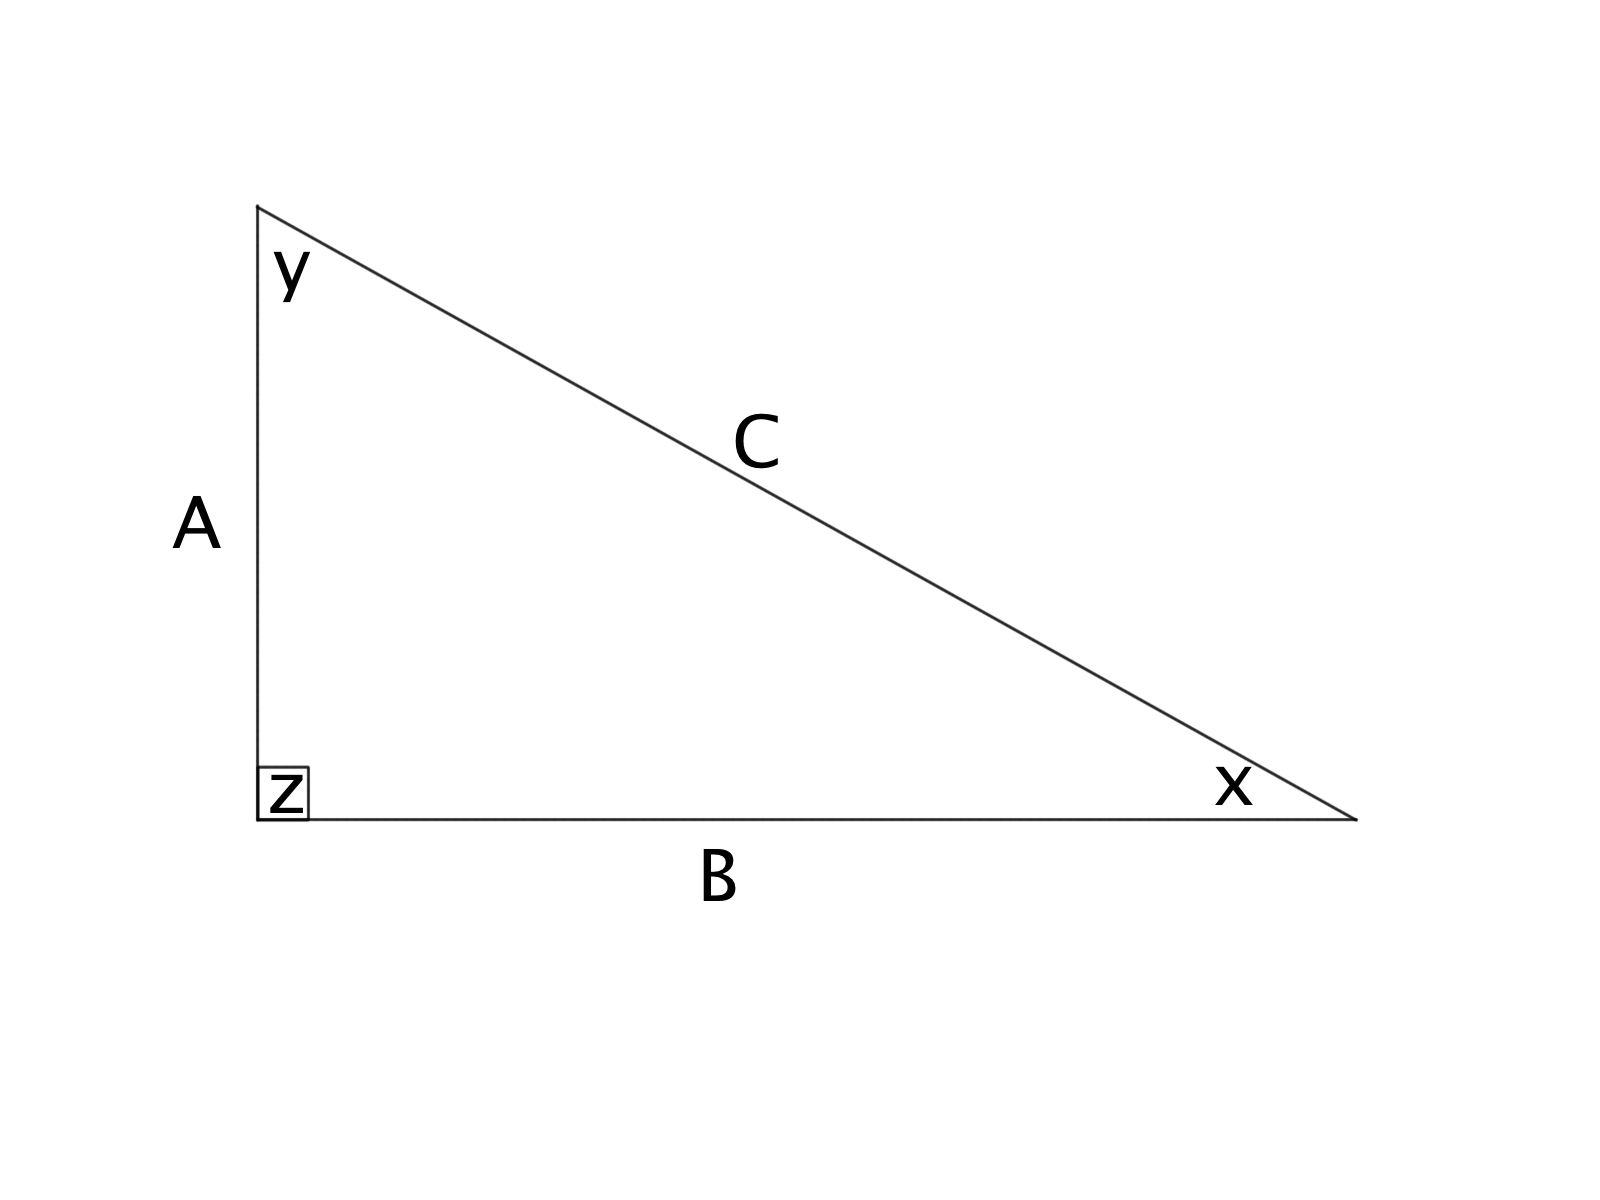
\includegraphics[width=5cm]{figures/triangle.jpg}
%    \caption[Placeholder]{Placeholder figure.}\label{fig:first}
%  \end{center}
%\end{figure}

%\begin{table}[h]                        
%  \begin{center}                          
%    \begin{tabular}{r|c|c}                  
%      \hline \hline                           
%      $(1,1)$ & $(1,2)$ & $(1,3)$\\           
%      \hline                                  
%      $(2,1)$ & $(2,2)$ & $(2,3)$\\           
%      \hline                                  
%      $(3,1)$ & $(3,2)$ & $(3,3)$\\
%      \hline \hline                           
%    \end{tabular}
%    \caption[Placeholder Table]{Placeholder table.}\label{tab:uno}
%  \end{center}
%\end{table}




%%%%%%%%%%%%%%%%%%%%%%%%%%%%%%%%%%%%%%% ACKNOWLEDGEMENTS %%%%%%%%%%%%%%%%%%%%%%%%%%%

\chapter*{Acknowledgements}

\thispagestyle{empty}

I wish to acknowledge the essential role my advisor Professor F. Zanasi has had in guiding me through the process of writing this thesis. He introduced me to applied category theory, to machine learning, and to the world of academic research, and I will be forever grateful for it. I also wish to thank my family and my friends, who supported my throughout this journey, and without whom all of this would not have been possible. To all of you, my most sincere gratitude.



\end{document}
